\documentclass[a4paper,11pt]{article}
\newcommand{\todo}[1]{{\tt $\ldots$ #1 $\ldots$ }}
\usepackage[utf8]{inputenc}  % Linux, macOS: enable non-English characters
%\usepackage[latin1]{inputenc}    % Windows: enable non-English characters
\usepackage[british]{babel}
\usepackage{fullpage}

\usepackage{amsmath}
\usepackage{amssymb}
\usepackage{amsthm} \newtheorem{theorem}{Theorem}
\usepackage{booktabs}
%\usepackage{clrscode3e}
\usepackage{color}
\usepackage{courier} % \texttt{...} gives thinner text
\usepackage{float}
\usepackage{mathtools} \mathtoolsset{showonlyrefs}  % provides \coloneqq
\usepackage{multirow}
\usepackage{tikz} \usetikzlibrary{trees}
\usepackage{listings}
\lstset{language=Python,
	basicstyle=\footnotesize\ttfamily,
	keywordstyle=\color[rgb]{0,0.5,0}\ttfamily,
	stringstyle=\color{orange}\ttfamily,
	commentstyle=\color{red}\ttfamily,
	tabsize=2,
	numbers=left, numberstyle=\tiny, numbersep=5pt,
	breaklines=true,
	breakatwhitespace=true,
	prebreak={/},
	captionpos=b,
	columns=fullflexible,
	escapeinside={\#*}{\^^M},
	mathescape
}
\usepackage{hyperref}  % should always be the last package


% useful wrappers for algorithmic/Python notation:
\newcommand{\length}[1]{\text{len}(#1)}
\newcommand{\twodots}{\mathinner{\ldotp\ldotp}}  % taken from clrscode3e.sty
\newcommand{\Returns}{\longrightarrow}

%% useful (wrappers for) math symbols:
\newcommand{\Cardinality}[1]{\left\lvert#1\right\rvert}
%\newcommand{\Cardinality}[1]{\##1}
\newcommand{\Ceiling}[1]{\left\lceil#1\right\rceil}
\newcommand{\Floor}[1]{\left\lfloor#1\right\rfloor}
\newcommand{\Iff}{\Leftrightarrow}
\newcommand{\Implies}{\Rightarrow}
\newcommand{\Intersect}{\cap}
\newcommand{\Oh}[1]{\mathcal{O}\left(#1\right)}
\newcommand{\Sequence}[1]{\left[#1\right]}
\newcommand{\Set}[1]{\left\{#1\right\}}
\newcommand{\SetComp}[2]{\Set{#1\SuchThat#2}}
\newcommand{\SuchThat}{\mid}
\newcommand{\Tuple}[1]{\langle#1\rangle}
\newcommand{\Union}{\cup}

%% fancy characters:
\usepackage{pifont}
%\newcommand{\scissors}{\ding{36}}
%\newcommand{\phone}{\ding{37}}
%\newcommand{\aircraft}{\ding{40}}
%\newcommand{\envelope}{\ding{41}}
\newcommand{\handpoint}{\ding{43}}
%\newcommand{\victory}{\ding{44}}
%\newcommand{\handwrite}{\ding{45}}
%\newcommand{\tick}{\ding{51}}
%\newcommand{\notick}{\ding{55}}

\renewcommand{\thepart}{\arabic{part}}
\renewcommand{\thesection}{\Alph{section}}

\title{\textbf{Algorithms \& Data Structures II (course 1DL231) \\
    Uppsala University -- Autumn 2019 \\
    Report for Assignment n  %% Replace n by 1, 2, or 3
    by Team t}}              %% Replace t by your team number

%% Replace by your name(s) and choose the encoding of line 3 or line 4:
\author{Clara CLÄVER \and Whiz KIDD}

%\date{Month Day, Year}
\date{\today}

\begin{document}

\maketitle

%% Delete this paragraph:
\noindent
This document shows the ingredients of a good assignment report for
this course.  The \LaTeX\ source code of this document illustrates
almost everything you need to know about \LaTeX\ in order to typeset a
professional-looking assignment report (for this course).  Use it as a
starting point for imitation and delete everything irrelevant.  The
usage of \LaTeX\ is \emph{optional}, but highly recommended, for
reasons that will soon become clear to those who have never used it
before; any learning time is \emph{outside} the budget of this course,
but will hugely pay off, if not in this course then in the next
course(s) you take and when writing a thesis or other scientific
report.

\part{Insertion Sort}\label{part:isort}
\setcounter{section}{0} % reset the section counter for each part/problem

\textsc{Insertion-Sort}\footnote{Your report need not contain an
  explanation, like in this paragraph, of the problem to be solved:
  you can start with the task answers, assuming the reader has read
  the problem statement in the assignment.} ``is an efficient
algorithm for sorting a small number of elements.  Insertion sort
works the way many people sort a hand of playing cards.  We start with
an empty left hand and the cards face down on the table.  We then
remove one card at a time from the table and insert it into the
correct position in the left hand.  To find the correct position for a
card, we compare it with each of the cards already in the hand, from
right to left, as illustrated in Figure~\ref{fig:isort}.  At all
times, the cards held in the left hand are sorted, and these cards
were originally the top cards of the pile on the table.'' (Quoted from
page~17 of CLRS3~\cite{CLRS}.)

\begin{figure}[t]  % make it float to the top of a page
  \centering
  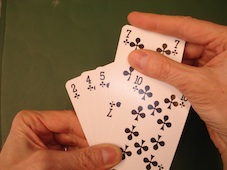
\includegraphics[height=6cm]{isort}
  \caption{Sorting a hand of cards using insertion sort.
    (\copyright\ nobody, 2010)}
  \label{fig:isort}
\end{figure}

\medskip

In the sequel of part~\ref{part:isort}, assume that the problem tasks in
the assignment were as follows (actual assignment statements in this
course may have other tasks):
\begin{enumerate}
\renewcommand{\theenumi}{\Alph{enumi}}
\item Implement \textsc{Insertion-Sort} as a Python function
  $\mathit{insertion\_sort}(A)$, where the elements to be sorted are
  provided in an integer array $A$ indexed from $0$ to $n-1$.  The
  sorting is to be done \emph{in place}, returning $A$ in
  non-decreasing order, that is:
  $A[0] \leq A[1] \leq \dots \leq A[n-1]$.  For brevity, you can refer
  to a sequence in non-decreasing order as a \emph{sorted sequence}.
\item Compute the best, average, and worst-case time complexities of
  \textsc{Insertion-Sort}.
\end{enumerate}

\section{Specification and Program}
\label{sec:pgm:isort}

A specification of sorting and our Python implementation of
\textsc{Insertion-Sort} are given in Listing~\ref{pgm:isort}, where
$n$ is referred to as $\length{A}$.

\lstinputlisting[firstline=11,lastline=30,firstnumber=11,
  %% See previous line for how only to include the actual contribution
  float=t,label=pgm:isort,caption={Python
  implementation of the \textsc{Insertion-Sort} algorithm on page~18
  of CLRS3~\cite{CLRS}. \handpoint~Compare for example
  line~\ref{line:ins-sort-while} with line~5 of that algorithm: arrays
  are indexed from~$1$ in CLRS3 but from~$0$ in Python.  Note also
  that a \emph{closed} interval $\ell \twodots u$, as used in the
  mathematical notation of the comments, is denoted by the
  \emph{right-open} interval $\ell : u+1$ in Python; you can use the
  Python notation in comments and the running text, as long as you
  comply with the Python semantics.}]{insertion_sort.py}

\section{Complexity Analysis}
\label{sec:analysis:isort}

The program in Listing~\ref{pgm:isort} has two nested loops, so we
analyse it starting from the inner loop, in
lines~\ref{line:ins-sort-while} to~\ref{line:ins-sort-while-end},
whose purpose is to insert $A[j]$ into the \emph{sorted} sequence
$A[0 \twodots j-1]$, assuming $j>0$, yielding the sorted sequence
$A[0 \twodots j]$.  Let $T_{\text{ins}}(j)$ denote the running time of
this inner loop:
\begin{equation} \label{rec:ins}
  T_{\text{ins}}(j) =
  \begin{cases}
    \Theta(1) & \text{if~} A[j-1] \leq A[j] \hfill \text{(best case)} \\
    \Theta(j) & \text{if~} A\left[\frac{j-1}{2}\right] < A[j] \leq
    A\left[\frac{j+1}{2}\right] \hfill ~~ (\text{if~} j>1) ~~~ \text{(average case)} \\
    \Theta(j) & \text{if~} A[j] < A[0] \hfill \text{(worst case)}
  \end{cases}
\end{equation}
assuming that every comparison takes constant time and every
assignment takes constant time.

We can now analyse the outer loop, and hence the whole algorithm.  Let
$n$ denote $\length{A}$ and let $T(n)$ denote the running time of
$\text{insertion\_sort}(A)$.  We get the following recurrence:
\begin{equation*}
  T(n) =
  \begin{cases}
    \Theta(1) & \text{if~} n < 2 \\
    T(n-1) + T_{\text{ins}}(n) & \text{if~} n \geq 2
  \end{cases}
\end{equation*}
Using recurrence~(\ref{rec:ins}), we get the following time complexity
results:
\begin{itemize}
\item $T(n) = \Theta(n)$ in the \emph{best case}, where the array is
  already non-decreasingly ordered before the sorting, so that
  $T_{\text{ins}}(n) = \Theta(1)$ at \emph{every} iteration of the
  outer loop, because $A[j]$ is always kept by the inner loop
  \emph{behind} the sorted sequence $A[0 \twodots j-1]$.  This result
  follows from Theorem~\ref{thm:ind} below, for the constants $a=1$
  and $b=2$.
\item $T(n) = \Theta(n^2)$ in the \emph{average case}, defined here as
  follows: \emph{on average} over the iterations of the outer loop,
  the inner loop inserts $A[j]$ into the \emph{middle} of the sorted
  sequence $A[0 \twodots j-1]$, so that $T_{\text{ins}}(n) =
  \Theta(n)$ on average at \emph{every} iteration of the outer loop.
  This can be proven by induction: $\langle$insert your proof
  here$\rangle$.
\item $T(n) = \Theta(n^2)$ in the \emph{worst case}, where the array
  is non-\emph{increasingly} ordered before the execution of the
  algorithm, so that $T_{\text{ins}}(n) = \Theta(n)$ at \emph{every}
  iteration of the outer loop, because $A[j]$ is always inserted by
  the inner loop at the \emph{beginning} of the sorted sequence $A[0
  \twodots j-1]$.  This result has the same proof as in the average
  case above.
\end{itemize}
In conclusion, \textsc{Insertion-Sort} takes $\Oh{n^2}$ time for an
array of $n$ elements.

\begin{theorem}
  \label{thm:ind}
  The following recurrence, for some \emph{constants} $a$ and $b$:
  \[
  T(n) =
  \begin{cases}
    \Theta(1) & \text{if~} n < b \\
    a \cdot T(n-1) + \Theta(1) & \text{if~} n \geq b
  \end{cases}
  \]
  has $\Theta(n)$ as closed form for $a = 1$, and $\Theta(a^n)$ as
  closed form for $a > 1$.
\end{theorem}

\begin{proof}
  By induction (left as an exercise to the reader in the AD1 course).
\end{proof}

\part{Weighted Interval Scheduling}\label{part:dp}
\setcounter{section}{0} % reset the section counter for each part/problem

\begin{quote}
``Suppose we have a set $S = \Set{a_1, a_2, \dots, a_n}$ of $n$ proposed
\emph{activities} that wish to use a resource, such as a lecture hall,
which can serve only one activity at a time. Each activity $a_i$ has a
\emph{start time} $s_i$ and a finish time $f_i$ , where
$0 \leq s_i < f_i < \infty$. If selected, activity $a_i$ takes place
during the half-open time interval $[s_i, f_i)$. Activities $a_i$ and
$a_j$ are \emph{compatible} if the intervals $[s_i, f_i)$ and
$[s_j, f_j)$ do not overlap. That is, $a_i$ and $a_j$ are compatible if
$s_i \geq f_j$ or $s_j \geq f_i$. In the 
\emph{activity-selection problem}, we wish to select a maximum-size
subset of mutually compatible activities.''
\end{quote}
(Quoted from page~415 of
CLRS3~\cite{CLRS}.)

The weighted interval scheduling problem is an extension to the 
activity-selection problem where activity $a_i$ has the weight $w_i$ and
where an optimal solution is to be found. An optimal solution to the
weighted interval problem is a subset,
$O \subseteq \Set{a_1, a_2, \dots, a_n}$, where the total weights over
the selected activities, $\sum \SetComp{w_i}{a_i \in O}$, is maximised.

Additionally, the activities are sorted in non-decreasing order of
finish times: $f_1 \leq f_2 \leq \cdots \leq f_n$ and the help function
$p(i)$ gives the largest index $j < i$ such that activity $i$ and $j$ are
compatible:

\begin{equation} \label{dp:helpfun}
  p(i) = 
  \begin{cases}
	\mathop{\mathrm{arg\,max}}\limits_{j\in 1 \twodots i-1} ( s_i \geq f_j ) & \hfill \qquad \text{if } \exists j \in 1\twodots i-1 : s_i \geq f_j \\
	0 & \hfill \text{otherwise}
  \end{cases}
\end{equation}

\medskip

In the sequel of part~\ref{part:dp}, assume that the problem tasks in
the assignment were as follows (actual assignment statements in this
course may have other tasks):
\begin{enumerate}
\renewcommand{\theenumi}{\Alph{enumi}}
\item Give a recursive equation for a parameterised quantity after 
  stating its meaning in terms of all its parameters. Use the equation
  to justify that the problem has the optimal substructure property
  and overlapping subproblems, so that dynamic programming is applicable
  to it.
\item Motivate your choice between bottom-up iteration (for which you
  must argue for  the chosen nesting and iteration order of the loops)
  and top-down recursion for the Weighted Interval Scheduling Problem.
\end{enumerate}

\section{Recursive equation}
\label{sec:recursive:actsel}

The weighted interval scheduling problem can be represented by the following
recursive function:

\begin{equation} \label{dp:opt}
  OPT(i) =
  \begin{cases}
    0 & \hfill \text{if } i = 0 \\
    \max~\{~OPT(i - 1), w_i + OPT(p(i))~\} & \hfill \text{if } i > 0
  \end{cases}
\end{equation}

Given an instance of the Weighted Interval Scheduling problem with an optimal
solution $O$, $O \subseteq J$. The last activity, $a_n$, either belongs to
$O$, $a_n \in O$, or it does not, $a_n \notin O$. If $a_n$ belongs to $O$,
then all intervals not compatible with $a_n$,
$\SetComp{a_i}{i \in p(n)+1 \twodots n-1}$, do not belong to $O$.

Additionally, if $a_n$ belongs to $O$, then $O$ must include an optimal
solution, $O^\prime_{p(n)}$, to the subproblem
$\SetComp{a_i}{i \in 1 \twodots p(n)}$. If $O^\prime_{p(n)}$ is not optimal,
then $O^\prime_{p(n)}$ could be modified into a solution that is optimal
and where all activities are intrinsically compatible with $a_n$.

If $a_n$ does not belong in $O$, then $O$ is an optimal solution to the
subproblem $\SetComp{a_i}{i \in 1 \twodots n-1}$. The reasoning is
analogous: assume that $a_n \notin O$; so if $O$ is not an
optimal solution to the subproblem of activities
$\SetComp{a_i}{a_i \in 1 \twodots n-1}$, then $O$ could be modified into
a solution that is.

Deciding if $a_n$ is to belong in $O$ thus require an optimal solution to the
subproblems $\SetComp{a_i}{i \in 1\twodots j}$, with $j$ taking the value
between $1$ and $n$, $j \in 1 \twodots n$, proving that Weighted Interval
scheduling has optimal substructure.

Given the index $i$ of an activity $a_i$, the recursive equation~\ref{dp:opt}
returns the weight $0$ for index $0$, denoting an empty set of activities,
and otherwise the optimal solution to the two subproblems: when activity $a_i$ does
not belong to the optimal subproblem for the activities 
$\SetComp{a_k}{k \in 1 \twodots i-1}$, or the optimal solution to the
subproblem with activities $\SetComp{a_k}{k \in 1 \twodots p(i)}$ plus the additional
weight $w_i$.

There are some problem instances that have overlapping subproblems. For
example; given the activities $\Set{a_1, a_2, \dots, a_n}$, $p(i)=k$, and $k\geq 1$,
then the subproblem $\Set{a_1, a_2, \dots, a_k}$ will be calculated at least
two times, once when finding the optimal solution for the problem $OPT(n)$ and
once for the subproblem $OPT(k+1)$.

\section{Bottom-Up Iteration and Top-Down Recursion}
\label{sec:bottom-up-rec}

Given the reasoning and the recursive function in task~\ref{sec:recursive:actsel},
the optimal solution to each subproblem $S_i$, with $1 \leq i \leq n$
and $S_i=\Set{a_1, \dots, a_i}$, will be found, giving
bottom-up iteration and top-down recursion the same time complexity.
We have chosen the bottom-up iterative approach. Our program
uses a single loop where all activities are iterated over in
increasing order of their indices, where activity $a_i$ has index $i$.


\bibliographystyle{abbrv}
\bibliography{ad2}  % Add your references to the ad2.bib file

%% Comment away the following line before submitting:
%\clearpage
\section*{Checklist before Submitting}

In order to protect yourself against an unnecessary loss of points,
use the following checklist before submitting:
\begin{itemize}
\item Crosscheck your report against the assignment instructions.
\item {\color{red}Remember that when submitting you implicitly certify
    (a)~that your report and all its uploaded attachments were
    produced solely by your team, except where explicitly stated
    otherwise and clearly referenced, (b)~that each teammate can
    individually explain any part starting from the moment of
    submitting your report, and (c)~that your report and attachments
    are not freely accessible on a public repository.}
\item Crosscheck against the technical writing and \LaTeX\ advice
  below.  The \emph{English Style Guide} of UU at
  \url{https://mp.uu.se/en/web/info/stod/kommunikation-riktlinjer/sprak/eng-skrivregler}
  and the technical-writing \emph{Checklist \& Style Manual} of the
  Optimisation group at
  \url{http://optimisation.research.it.uu.se/checkList.pdf} offer many
  further pieces of advice.  Common errors in English usage are
  discussed at \url{https://brians.wsu.edu/common-errors}.  In
  particular, common errors in English usage by native Swedish
  speakers are listed at
  \url{http://www.crisluengo.net/index.php/english-language}.
\item Spellcheck all documents, including the comments in the source
  code.
\item Proofread, if not grammar-check, your report at least once per
  teammate.
\end{itemize}

\section*{More \LaTeX\ and Technical Writing Advice}

Unnumbered itemisation (only to be used when the order of the items
does \emph{not} matter):\footnote{Use footnotes very sparingly, and
  note that footnote pointers are \emph{never} preceded by a space and
  always glued immediately \emph{behind} the punctuation, if there is
  any.}
\begin{itemize}
\item Unnumbered displayed formula:
  \[
  E = m \cdot c^2
  \]
\item Numbered displayed formula, which is cross-referenced somewhere:
  \begin{equation}
    \label{eq:emc2}
    E = m \cdot c^2
  \end{equation}
\item Formula --- the same as formula~(\ref{eq:emc2}) --- spanning
  more than one line:
  \begin{gather*}
    E \\ = m \cdot c^2
  \end{gather*}  
\end{itemize}
Numbered itemisation (only to be used when the order of the items
\emph{does} matter):
\begin{enumerate}
\item First do this.
\item\label{item:that} Then do that.
\item If we are not finished, then go back to Step~\ref{item:that},
  else stop.
\end{enumerate}

Tables and elementary mathematics are typeset as given in
Table~\ref{tab:maths}; see
\url{ftp://ftp.ams.org/pub/tex/doc/amsmath/short-math-guide.pdf} for
many more details.


Use \verb|\mathit{...}| in mathematical mode for each multiple-letter
identifier in order to avoid typesetting the identifier like the
product of single-letter ones.  For example, note the typographic
difference between the identifier $\mathit{WL}$, obtained through
\verb|$\mathit{WL}$|, and the product $WL$, where there is a small
space between the $W$ and the $L$, obtained through \verb|$WL$|.

Do \emph{not} use programming-language-style lower-ASCII notation
(such as $!$ for negation, $\&\&$ for conjunction, $||$ for
disjunction, and the equality sign $=$ for assignment) in algorithms
or formulas (but rather use $\neg$ or $\mathbf{not}$, $\land$ or $\&$
or $\mathbf{and}$, $\lor$ or $\mathbf{or}$, and $\gets$ or
$\coloneqq$, respectively), as this testifies to a very strong
confusion of concepts.

Figures can be imported with \verb|\includegraphics|
% (such as Figure~\ref{fig:demo})
or drawn inside the \LaTeX\ source code using the highly declarative
notation of the \texttt{tikz} package: see Figure~\ref{fig:trees} for
sample drawings.  It is perfectly acceptable in this course to include
scans or photos of drawings that were carefully done by hand.

%\begin{figure}[t] % make it float towards the top of a page
%  \centering
%  \includegraphics[height=5cm]{lulu.jpg}
%  \caption{The text under the figure}
%  \label{fig:demo}
%\end{figure}

\begin{figure}[t] % make it float to the top of a page
  \begin{center}
    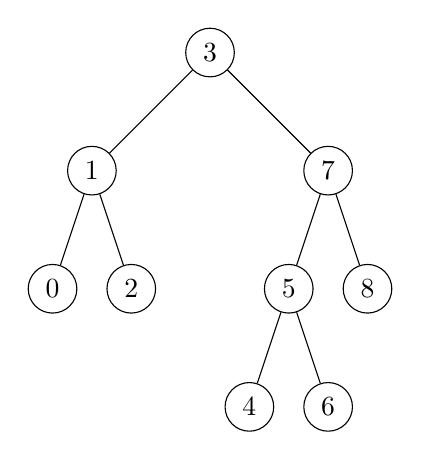
\begin{tikzpicture}
      [level 1/.style={sibling distance=30mm},
       level 2/.style={sibling distance=15mm},
       level 2/.style={sibling distance=10mm}]
      \tikzstyle{every node}=[circle,draw]
      \node{3}
      child{
        node{1}
        child{node{0}}
        child{node{2}}
      }
      child{
        node{7}
        child{
          node{5}
          child{node{4}}
          child{node{6}}
        }
        child{node{8}}
      };
    \end{tikzpicture} \hspace{4mm}
    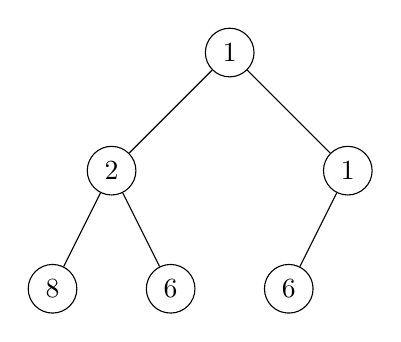
\begin{tikzpicture}
      [level 1/.style={sibling distance=30mm},
       level 2/.style={sibling distance=15mm}]
      \tikzstyle{every node}=[circle,draw]
      \node{1}
      child{
        node{2}
        child{node{8}}
        child{node{6}}
      }
      child{
        node{1}
        child{node{6}}
        child[missing]{node{k}}
      }
      ;
    \end{tikzpicture} \hspace{4mm}
    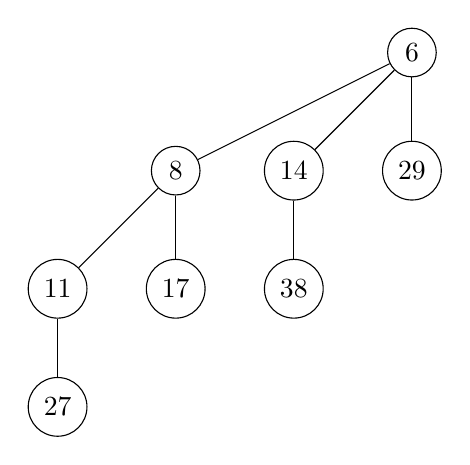
\begin{tikzpicture}[grow via three points={%
        one child at (0,-1.5) and two children at (0,-1.5) and (-1.5,-1.5)}]
      \tikzstyle{every node}=[circle,draw]
      \node at (0,0) {6}
      child{node{29}}
      child{
        node{14}
        child{
          node{38}
        }
      }
      child{
        node{8}
        child{node{17}}
        child{
          node{11}
          child{node{27}}
        }
      }
      ;
    \end{tikzpicture}
  \end{center}
  \caption{A binary search tree (on the left), a binary min-heap (in
    the middle), and a binomial tree of rank $3$ (on the right).}
  \label{fig:trees}
\end{figure}

If you are not sure whether you will stick to your current choice of
notation or terminology, then introduce a new (possibly parametric)
command.  For example, upon
\begin{center}
  \verb|\newcommand{\Cardinality}[1]{\left\lvert#1\right\rvert}|
\end{center}
the formula \verb|$\Cardinality{S}$| typesets the cardinality of set
$S$ as $\Cardinality{S}$ with autosized vertical bars and proper
spacing, but upon changing the definition of that parametric command
to
\begin{center}
  \verb|\newcommand{\Cardinality}[1]{\# #1}|
\end{center}
and recompiling, the formula \verb|$\Cardinality{S}$| typesets the
cardinality of set $S$ as $\#S$.
%
You can thus obtain an arbitrary number of changes in the document
with a \emph{constant}-time change in its source code, rather than
having to perform a \emph{linear}-time find-and-replace operation
within the source code, which is painstaking and error-prone.  The
source code of this document has some useful predefined commands about
mathematics and algorithms.

Use commands on positioning (such as \verb|\hspace|, \verb|\vspace|,
and \verb|\noindent|) and appearance (such as \verb|\small| for
reducing the font size, and \verb|\textit| for italics) very
sparingly, and ideally only in (parametric) commands, as the very idea
of mark-up languages such as \LaTeX\ is to let the class designer
(usually a trained professional typesetter) decide on where things
appear and how they look.  For example, \verb|\emph| (for emphasis)
compiles (outside italicised environments, such as \texttt{theorem})
into \textit{italics} under the \texttt{article} class used for this
document, but it may compile into \textbf{boldface} under some other
class.
\begin{center}
  \textbf{If you do not (need to) worry about \emph{how} things look, \\
    then you can fully focus on \emph{what} you are trying to
    express!}
\end{center}

Note that \emph{no} absolute numbers are used in the \LaTeX\ source
code for any of the references inside this document.  For ease of
maintenance, \verb|\label| is used for giving a label to something
that is automatically numbered (such as an algorithm, equation,
figure, footnote, item, line, part, section, subsection, or table),
and \verb|\ref| is used for referring to a label.  An item in the
bibliography file is referred to by \verb|\cite| instead.  Upon
changing the text, it suffices to recompile, once or twice, and
possibly to run BibTeX again, in order to update all references
consistently.

Always write
%
\verb| Table|$\sim$\verb|\ref{tab:maths} |
%
instead of
%
\verb| Table \ref{tab:maths}|,
%
by using the non-breaking space (which is typeset as the tilde $\sim$)
instead of the normal space, because this avoids that a
cross-reference is spread across a line break, as for example in
``Table \ref{tab:maths}'', which is considered poor typesetting.

The rules of English for how many spaces to use before and after
various symbols are given in Table~\ref{tab:spacing}.  Beware that
they may be very different from the rules in your native language.

\begin{table}
  \centering
  \begin{tabular}{|c|c|c|c|}
    \cline{3-4}
    \multicolumn{2}{c|}{} & \multicolumn{2}{c|}{number of spaces after} \\
    \cline{3-4}
    \multicolumn{2}{c|}{} & 0 & 1 \\
    \hline
    \multirow{2}{*}{number of spaces before} & 0 & / - & , : ; . ! ?
    ) ] \} ' '' \% \\
    \cline{2-4}
    & 1 & ( [ \{ ` `` & -- (\emph{n}-dash) --- (\emph{m}-dash) \\
    \hline
  \end{tabular}
  \caption{Spacing rules of English}
  \label{tab:spacing}
\end{table}

%\newpage

\begin{table}%[t] % make it float to the top of a page
  \centering
  \begin{tabular}{rlc} % right left centre
    \toprule
    Topic & \LaTeX\ code & Appearance \\
    \midrule
    Greek letter & \verb|$\Theta,\Omega,\epsilon$| & $\Theta,\Omega,\epsilon$ \\
    multiplication & \verb|$m \cdot n$| & $m \cdot n$ \\
    division & \verb|$\frac{m}{n}, m \div n$| & $\frac{m}{n}, m \div n$ \\
    rounding down & \verb|$\left\lfloor n \right\rfloor$| & $\left\lfloor n \right\rfloor$ \\
    rounding up & \verb|$\left\lceil n \right\rceil$| & $\left\lceil n \right\rceil$ \\
    binary modulus & \verb|$m \bmod n$| & $m \bmod n$ \\
    unary modulus & \verb|$m \equiv n \mod \ell$| & $m \equiv n \mod \ell$ \\
    root & \verb|$\sqrt{n},\sqrt[3]{n}$| & $\sqrt{n},\sqrt[3]{n}$ \\
    exponentiation, superscript & \verb|$n^{i}$| & $n^{i}$ \\
    subscript & \verb|$n_{i}$| & $n_{i}$ \\
    overline & \verb|$\overline{n}$| & $\overline{n}$ \\
    base $2$ logarithm & \verb|$\lg n$| & $\lg n$ \\
    base $b$ logarithm & \verb|$\log_b n$| & $\log_b n$ \\
    binomial & \verb|$\binom{n}{k}$| & $\binom{n}{k}$ \\
    sum & \verb|\[\sum_{i=1}^n i\]| & $\displaystyle\sum_{i=1}^n i$ \\
    numeric comparison & \verb|$\leq,<,=,\neq,>,\geq$| & $\leq,<,=,\neq,>,\geq$ \\
    non-numeric comparison & \verb|$\prec,\nprec,\preceq,\succeq$| & $\prec,\nprec,\preceq,\succeq$ \\
    extremum & \verb|$\min,\max,+\infty,\bot,\top$| & $\min,\max,+\infty,\bot,\top$ \\
    function & \verb|$f\colon A\to B,\circ,\mapsto$| & $f\colon A\to B,\circ,\mapsto$ \\
    sequence, tuple & \verb|$\langle a,b,c \rangle$| & $\langle a,b,c \rangle$ \\
    set & \verb|$\{a,b,c\},\emptyset,\mathbb{N}$| & $\{a,b,c\},\emptyset,\mathbb{N}$ \\
    set membership & \verb|$\in,\not\in$| & $\in,\not\in$ \\
    set comprehension & \verb|$\{i \mid 1 \leq i \leq n\}$| & $\{i \mid 1 \leq i \leq n\}$ \\
    set operation & \verb|$\cup,\cap,\setminus,\times$| & $\cup,\cap,\setminus,\times$ \\
    set comparison & \verb|$\subset,\subseteq,\not\supset$| & $\subset,\subseteq,\not\supset$ \\
    logic quantifier & \verb|$\forall,\exists,\nexists$| & $\forall,\exists,\nexists$ \\
    logic connective & \verb|$\land,\lor,\neg,\Rightarrow$| & $\land,\lor,\neg,\Rightarrow$ \\
    logic & \verb|$\models,\equiv,\vdash$| & $\models,\equiv,\vdash$ \\
    miscellaneous & \verb|$\&,\#,\approx,\sim,\ell$| & $\&,\#,\approx,\sim,\ell$ \\
    dots & \verb|$\ldots,\cdots,\vdots,\ddots$| & $\ldots,\cdots,\vdots,\ddots$ \\
    dots (context-sensitive) & \verb|$1,\dots,n; 1+\dots+n$| & $1,\dots,n; 1+\dots+n$ \\
    parentheses (autosizing) & \verb|$\left(m^{n^k}\right),(m^{n^k})$| & $\left(m^{n^k}\right),(m^{n^k})$ \\
    identifier of $>1$ character & \verb|$\mathit{identifier}$| & $\textit{identifier}$ \\
    hyphen, \emph{n}-dash, \emph{m}-dash, minus & \verb|-|, \verb|--|, \verb|---|, \verb|$-$| & -, --, ---, $-$ \\
    \bottomrule
  \end{tabular}
  \caption{The typesetting of elementary mathematics.  Note very carefully
    when italics are used by \LaTeX\ and when not, as well as all the
    horizontal and vertical spacing performed by \LaTeX.}
  \label{tab:maths}
\end{table}

%\newpage


%\vfill

%\noindent
%\handpoint\ Feel free to report to the head teacher any other features
%that you would have liked to see discussed and exemplified in this
%template document.


\end{document}

%%% Local Variables:
%%% mode: latex
%%% TeX-master: t
%%% End:
